\section{Experiments}

\subsection{Implementation Details}

In our experiments, we adhere to the protocols outlined in the commonly used BasicLFSR framework \cite{BasicLFSR} for implementing and benchmarking M2MT-Net. Five public datasets are used, namely \textit{EPFL} \cite{rerabekEPFL2016}, \textit{HCInew} \cite{honauerHCInew_ACCV2016}, \textit{HCIold} \cite{wannerHCIold_VMV2013}, \textit{INRIA} \cite{lependuINRIA_TIP2018}, and \textit{STFgantry} \cite{vaishSTFgantry_2008}. These datasets contain 70/20/10/35/9 samples for training and 10/4/2/5/2 samples for testing. Following the protocols, we only use the central $5 \times 5$ SAIs \cite{BasicLFSR}. For training, each SAI was partitioned into $64 \times 64$ or $128 \times 128$ patches to serve as HR patches, and $1/2$ or $1/4$ bicubic down-sampling is applied to produce the corresponding LR patches for $2 \times$ or $4 \times$ scales, respectively. We use Adam optimizer with a learning rate of $2 \times 10^{-4}$ and batches of 4 samples. The training process takes 100 epochs to sufficiently converge. Regarding the hyperparameters, we use $C=48$ across all Transformers and convolutions except Correlation Tensors with $C_{Cor} = 128$. The number of initial spatial convolutions is set to 4, and the number of correlation blocks $n_2$ is set to 8.

The experiments are conducted on a desktop computer with an Intel i7-11700 4.800GHz 8-core CPU, 32 MB RAM, and an Nvidia GTX 3090 GPU. We implement M2MT-Net using the PyTorch framework. The implementation code and trained models will be released publicly.

\subsection{Quantitative Comparisons}
A quantitative comparison is conducted to compare M2MT-Net with eight state-of-the-art LFSR methods on the five aforementioned datasets at $2 \times$ and $4 \times$ scales. The compared methods include convolution-based LFSSR \cite{yeungSAS_LFSR2019}, LF-ATO \cite{jinLFSSRATO_2020}, LF-InterNet \cite{wangLfInterNet_ECCV2020}, LF-IINet \cite{liuLFIINet_TMM2021}, DKNet \cite{huDKNet_TIM2022}, DistgSSR \cite{wangDistgSSR_TIP2022}, and Transformer-based methods DPT \cite{wangDPT_AAAI2022}, LFT \cite{liangLFT_SPL2022}, and EPIT \cite{liangEPIT_arXiv2023}. The outcomes are presented in Table \ref{tab:overall}.

It is evident that our M2MT-Net holds a superior position. At both the $2 \times$ and $4 \times$ scales, it achieves the highest PSNR across datasets. Notably, on the \textit{EPFL} dataset, which contains the most testing samples, M2MT-Net surpasses the second-best method, EPIT, by a significant 0.53 dB PSNR gain at the $2 \times$ scale and 0.46 dB at the $4 \times$ scale. M2MT-Net ranks second to EPIT in only one dataset, namely \textit{STFgantry}. This particular outcome can be attributed to the dataset's distinctive characteristic of exhibiting high disparities, a feature effectively managed by EPIT due to its utilization of the EPI mechanism.

A discernible trend is observed regarding the performance of Transformer-based methods on the \textit{EPFL} dataset, such as LFT and EPIT, in comparison to convolutional methods, with DistgSSR as the representative. At the $2 \times$ scale, the superiority of EPIT over DistgSSR is marginal, by just 0.02 dB, with LFT trailing further. Yet, at the $4 \times$ scale, both LFT and EPIT remarkably outdo DistgSSR by margins of 0.35 dB and 0.27 dB, respectively. This discrepancy underscores the inherent strengths of convolutions in extracting high-frequency information, particularly visual textures, which become advantageous at the $2 \times$ scale where most lost visual textures are still recoverable. Conversely, Transformers excel in modeling distant pixel or SAI dependencies, rendering them more suitable for the $4 \times$ scale where a model has to utilize existing spatial and angular cues more effectively. Different from LFT and EPIT, M2MT-Net, with the subspace isolation mitigated, integrates the advantages of both methodologies, thereby achieving significant lead margins of 0.55 dB and 0.81 dB over DistgSSR on the \textit{EPFL} dataset at both scales.

We also incorporate the geometric self-ensemble strategy, which was initially proposed for single image super-resolution \cite{limEDSR_CVPRW2017}, into M2MT-Net to enhance the model performance without introducing additional parameters. The variant is labeled as M2MT-Net* in Table \ref{tab:overall}. Similar to its application in 2D single images, during inference, the strategy transforms the 2D LR by flipping and rotating to construct an ensemble ${T_{i}\overline{I}_{LR}}$, where $T_{i}$ represents a transform function. The SR is generated by executing the network on each member in the ensemble individually, followed by the corresponding inverse transform, and finally averaging the output. The strategy is expressed as
\begin{equation}
    I_{SR} = \frac{1}{n} \sum_{i = 1}^{n} T_{i}^{-1}\mathcal{F}(T_{i}(I_{LR}))
\end{equation}
where $n$ is the number of transforms. Given that these transforms operate on the reshaped 2D SAI-view LF $\overline{I}_{LR} \in \mathbb{R}^{U V \times WH \times C}$, they take effect on both the spatial and angular spaces synergistically, ensuring the LF structure is not distorted but preserved after transform. The result in Table \ref{tab:overall} demonstrates the advantageous impact brought by the strategy with a roughly 0.10 to 0.25 dB increase in PSNR observed across the datasets and a particular 0.43 dB and 0.32 dB increase on the \textit{STFgantry} dataset at the $2 \times$ and $4 \times$ scales respectively. These findings suggest that the geometric self-ensemble strategy is a valuable addition to compensate and enhance LFSR models.


\subsection{Qualitative Comparisons}
We further explore the superior performance of LF-SANet in qualitative evaluation. Figure \ref{fig:Qual} presents qualitative results at the $4 \times$ scale for three representative samples, namely (a) \textit{Perforated\_Metal\_3}, (b) \textit{Palais\_du\_Luxembourg} and (c) \textit{Bicycle}. The first two samples are from the \textit{EPFL} dataset captured by Lytro cameras \cite{Lytro}, and the third one is from the synthetic dataset \textit{HCInew}. We compared M2MT-Net with four other methods: IINet and DistgSSR represent the convolution-based methods, while LFT and EPIT are from the Transformer-based group. Zoom-in views inside blue and red boxes are provided to show more details. Accompanying these visuals, PSNR/SSIM calculated on the red box areas. In general, all these techniques capably enhance resolution and preserve primary structures, but nuanced distinctions emerge within the details, especially the zoom-in views of red boxes.

In the \textit{Perforated\_Metal\_3} sample, most methods portray the perforated hole reasonably well but fall short in edge sharpness, likely influenced by lighting and occlusion challenges. M2MT-Net, however, produces notably sharper edges and more round shape of the hole. In the \textit{Palais\_du\_Luxembourg} sample, M2MT-Net excels in reconstructing the textures of the bricks beyond the other methods. For the \textit{Bicycle} sample, the edges of the books are clearly sharper in M2MT-Net than others.

In Figure \ref{fig:QualMatrix}, SAI-wise PSNR on these three samples is visualized. The visual representation highlights M2MT-Net's notable enhancements across SAIs. Notably, in cases (a) \textit{Perforated\_Metal\_3} and (c) \textit{Bicycle}, the lowest PSNR values achieved by M2MT-Net are still higher than the highest PSNR values of other methods. This signifies the consistent superiority of M2MT-Net.

\subsection{LAM Analysis} To further probe into the underlying capability of M2MT-Net, we employ the Local Attribution Map (LAM) technique \cite{guLAM_CVPR2021} to discern influential pixels, thereby providing insight and transparency into the performance of M2MT-Net. In Figure \ref{fig:Qual}, the LAM visualization is provided below PSNR/SSIM. It is calculated on the blue box regions with the red box regions as targets. Diffusion Index (DI) accompanies the visualization as a qualitative indicator of pixel utilization.

From the results, M2MT-Net's superior utilization across the three samples is evident, demonstrating significantly more active pixels both within and across SAIs. This superiority is further supported by the DI values as M2MT-Net consistently records values above 20, while competing methods hover at 10 or even lower. Delving deeper into these active pixels reveals intriguing insights.

For instance, in the \textit{Perforated\_Metal\_3} sample, though repeated perforated holes offer potential patterns for reconstruction, most methods focus solely on the neighboring area. In contrast, M2MT-Net's active pixels span the entire column, suggesting that it identifies shared characteristics among the holes in the column and leverages them as complementary cues. 
Similarly, in the \textit{Palais\_du\_Luxembourg} sample, the texture of brick walls exhibit recurring patterns for reuse. M2MT-Net manages to utilize not only the specific brick wall but also the neighboring one on the right, and the influential pixels have high activities across SAIs, hence the patterns are recovered with visible edges, unlike its counterparts generate a blurry area due to their narrower focus and weaker correlation across SAIs.
For the \textit{Bicycle} sample, the books on the shelves present similar patterns as well. M2MT-Net's advantage becomes evident as it activates pixels not only around the local area but also on a book in a similar red color on the shelf above, regardless of the distance.

The DI values offer insights into the relationship between model performance and pixel utilization. In theory, higher DI indicates better pixel utilization and should result in improved performance. This holds true for M2MT-Net, as it achieves a double-digit DI alongside significantly higher PSNR and SSIM scores, and it still holds true if comparing only within the convolution-based or Transformer-based groups.

The DI values shed light on the relation between model performance and pixel utilization. In theory, higher DI indicates higher pixel utilization and should result in better performance. It holds true for M2MT-Net as having a double-digit DI and a significantly higher PSNR and SSIM, and it remains consistent when comparing only within the convolution-based or Transformer-based groups. However, when comparing across these two groups, a different trend emerges as convolution-based IINet and DistgSSR tend to have higher DI values but often lag behind Transformer-based LFT and EPIT in terms of PSNR and SSIM. This highlights the distinct nature of pixel utilization between convolutions and Transformers, where convolutions leverage more pixels but are constrained by locality, while Transformers use fewer pixels in a more effective way through its global dependency modeling mechanism.

\begin{figure*}[ht!]
    \centering
    \tabcolsep=0.05cm
    \renewcommand{\arraystretch}{1.0}
    {\small 
    \begin{tabular}{ccccccc}
    % Perforated_Metal_3
    \raisebox{-0.5\height}[0pt][0pt]{
        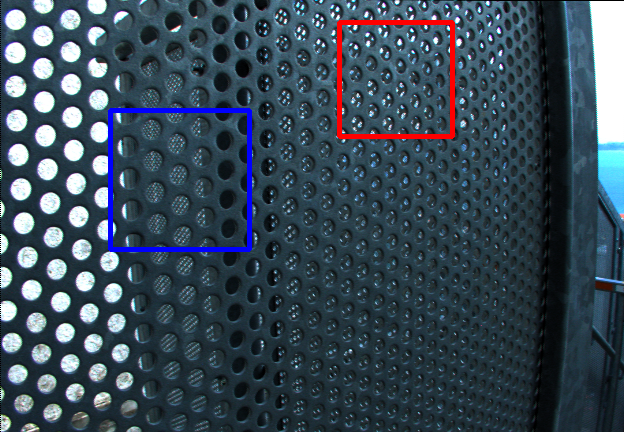
\includegraphics[width=0.25\textwidth, height=0.17\textwidth]{img/depth/full/Perforated_Metal_3/rgb_annotated.png}
    } &
    
\includegraphics[width=0.110\textwidth, height=0.110\textwidth,cfbox=blue 1pt 0pt]{img/depth/crop/Perforated_Metal_3/GT_1.png} &
    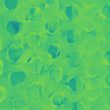
\includegraphics[width=0.110\textwidth, height=0.110\textwidth,cfbox=blue 1pt 0pt]{img/depth/crop/Perforated_Metal_3/IINet_1.png} &
    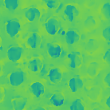
\includegraphics[width=0.110\textwidth, height=0.110\textwidth,cfbox=blue 1pt 0pt]{img/depth/crop/Perforated_Metal_3/DistgSSR_1.png} &
    
\includegraphics[width=0.110\textwidth, height=0.110\textwidth,cfbox=blue 1pt 0pt]{img/depth/crop/Perforated_Metal_3/LFT_1.png} &
    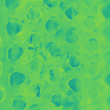
\includegraphics[width=0.110\textwidth, height=0.110\textwidth,cfbox=blue 1pt 0pt]{img/depth/crop/Perforated_Metal_3/EPIT_1.png} &
    
\includegraphics[width=0.110\textwidth, height=0.110\textwidth,cfbox=blue 1pt 0pt]{img/depth/crop/Perforated_Metal_3/SATNet_1.png} \\
    &
    
\includegraphics[width=0.110\textwidth, height=0.110\textwidth,cfbox=red 1pt 0pt]{img/depth/crop/Perforated_Metal_3/GT_2.png} &
    
\includegraphics[width=0.110\textwidth, height=0.110\textwidth,cfbox=red 1pt 0pt]{img/depth/crop/Perforated_Metal_3/IINet_2.png} &
    
\includegraphics[width=0.110\textwidth, height=0.110\textwidth,cfbox=red 1pt 0pt]{img/depth/crop/Perforated_Metal_3/DistgSSR_2.png} &
    
\includegraphics[width=0.110\textwidth, height=0.110\textwidth,cfbox=red 1pt 0pt]{img/depth/crop/Perforated_Metal_3/LFT_2.png} &
    
\includegraphics[width=0.110\textwidth, height=0.110\textwidth,cfbox=red 1pt 0pt]{img/depth/crop/Perforated_Metal_3/EPIT_2.png} &
    
\includegraphics[width=0.110\textwidth, height=0.110\textwidth,cfbox=red 1pt 0pt]{img/depth/crop/Perforated_Metal_3/SATNet_2.png} \\
    
    \textit{Perforated\_Metal\_3} &
    Ground-truth &
    IINet \cite{liuLFIINet_TMM2021} &
    DistgSSR \cite{wangDistgSSR_TIP2022} &
    LFT \cite{liangLFT_SPL2022} &
    EPIT \cite{liangEPIT_arXiv2023} &
    M2MT-Net \\

    MSE$\times100$ &
    &
    0.968 &
    \underline{0.832} &
    1.037 &
    0.918 &
    \textbf{0.706} \\

    \vspace{-5pt} \\

    % Sphynx
    \raisebox{-0.5\height}[0pt][0pt]{
        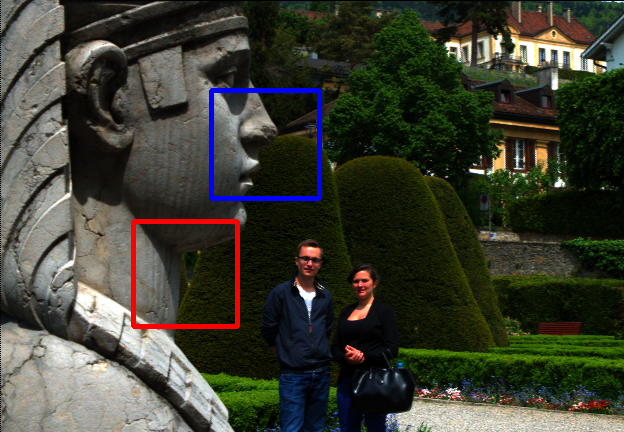
\includegraphics[width=0.25\textwidth, height=0.17\textwidth]{img/depth/full/Sphynx/rgb_annotated.png}
    } &
    
\includegraphics[width=0.110\textwidth, height=0.110\textwidth,cfbox=blue 1pt 0pt]{img/depth/crop/Sphynx/GT_1.png} &
    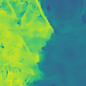
\includegraphics[width=0.110\textwidth, height=0.110\textwidth,cfbox=blue 1pt 0pt]{img/depth/crop/Sphynx/IINet_1.png} &
    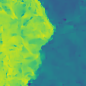
\includegraphics[width=0.110\textwidth, height=0.110\textwidth,cfbox=blue 1pt 0pt]{img/depth/crop/Sphynx/DistgSSR_1.png} &
    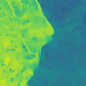
\includegraphics[width=0.110\textwidth, height=0.110\textwidth,cfbox=blue 1pt 0pt]{img/depth/crop/Sphynx/LFT_1.png} &
    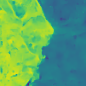
\includegraphics[width=0.110\textwidth, height=0.110\textwidth,cfbox=blue 1pt 0pt]{img/depth/crop/Sphynx/EPIT_1.png} &
    
\includegraphics[width=0.110\textwidth, height=0.110\textwidth,cfbox=blue 1pt 0pt]{img/depth/crop/Sphynx/SATNet_1.png} \\
    &
    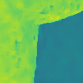
\includegraphics[width=0.110\textwidth, height=0.110\textwidth,cfbox=red 1pt 0pt]{img/depth/crop/Sphynx/GT_2.png} &
    
\includegraphics[width=0.110\textwidth, height=0.110\textwidth,cfbox=red 1pt 0pt]{img/depth/crop/Sphynx/IINet_2.png} &
    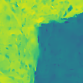
\includegraphics[width=0.110\textwidth, height=0.110\textwidth,cfbox=red 1pt 0pt]{img/depth/crop/Sphynx/DistgSSR_2.png} &
    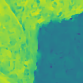
\includegraphics[width=0.110\textwidth, height=0.110\textwidth,cfbox=red 1pt 0pt]{img/depth/crop/Sphynx/LFT_2.png} &
    
\includegraphics[width=0.110\textwidth, height=0.110\textwidth,cfbox=red 1pt 0pt]{img/depth/crop/Sphynx/EPIT_2.png} &
    
\includegraphics[width=0.110\textwidth, height=0.110\textwidth,cfbox=red 1pt 0pt]{img/depth/crop/Sphynx/SATNet_2.png} \\
    
    \textit{Sphynx} &
    Ground-truth &
    IINet \cite{liuLFIINet_TMM2021} &
    DistgSSR \cite{wangDistgSSR_TIP2022} &
    LFT \cite{liangLFT_SPL2022} &
    EPIT \cite{liangEPIT_arXiv2023} &
    M2MT-Net \\

    MSE$\times100$ &
    &
    0.178 &
    \underline{0.139} &
    0.149 &
    0.147 &
    \textbf{0.136} \\

    \vspace{-5pt} \\

    % bicycle
    \raisebox{-0.5\height}[0pt][0pt]{
        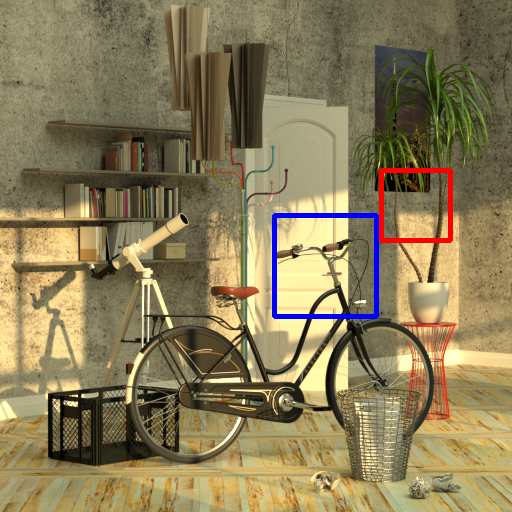
\includegraphics[width=0.22\textwidth, height=0.22\textwidth]{img/depth/full/bicycle/rgb_annotated.png}
    } &
    
\includegraphics[width=0.110\textwidth, height=0.110\textwidth,cfbox=blue 1pt 0pt]{img/depth/crop/bicycle/GT_1.png} &
    
\includegraphics[width=0.110\textwidth, height=0.110\textwidth,cfbox=blue 1pt 0pt]{img/depth/crop/bicycle/IINet_1.png} &
    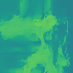
\includegraphics[width=0.110\textwidth, height=0.110\textwidth,cfbox=blue 1pt 0pt]{img/depth/crop/bicycle/DistgSSR_1.png} &
    
\includegraphics[width=0.110\textwidth, height=0.110\textwidth,cfbox=blue 1pt 0pt]{img/depth/crop/bicycle/LFT_1.png} &
    
\includegraphics[width=0.110\textwidth, height=0.110\textwidth,cfbox=blue 1pt 0pt]{img/depth/crop/bicycle/EPIT_1.png} &
    
\includegraphics[width=0.110\textwidth, height=0.110\textwidth,cfbox=blue 1pt 0pt]{img/depth/crop/bicycle/SATNet_1.png} \\
    &
    
\includegraphics[width=0.110\textwidth, height=0.110\textwidth,cfbox=red 1pt 0pt]{img/depth/crop/bicycle/GT_2.png} &
    
\includegraphics[width=0.110\textwidth, height=0.110\textwidth,cfbox=red 1pt 0pt]{img/depth/crop/bicycle/IINet_2.png} &
    
\includegraphics[width=0.110\textwidth, height=0.110\textwidth,cfbox=red 1pt 0pt]{img/depth/crop/bicycle/DistgSSR_2.png} &
    
\includegraphics[width=0.110\textwidth, height=0.110\textwidth,cfbox=red 1pt 0pt]{img/depth/crop/bicycle/LFT_2.png} &
    
\includegraphics[width=0.110\textwidth, height=0.110\textwidth,cfbox=red 1pt 0pt]{img/depth/crop/bicycle/EPIT_2.png} &
    
\includegraphics[width=0.110\textwidth, height=0.110\textwidth,cfbox=red 1pt 0pt]{img/depth/crop/bicycle/SATNet_2.png} \\
    
    \textit{bicycle} &
    Ground-truth &
    \small IINet \cite{liuLFIINet_TMM2021} &
    DistgSSR \cite{wangDistgSSR_TIP2022} &
    LFT \cite{liangLFT_SPL2022} &
    EPIT \cite{liangEPIT_arXiv2023} &
    M2MT-Net \\

    MSE$\times100$ &
    &
    2.805 &
    2.633 &
    2.652 &
    \underline{2.557} &
    \textbf{2.324} \\

    \vspace{-5pt} \\

    % monasRoom
    \raisebox{-0.5\height}[0pt][0pt]{
        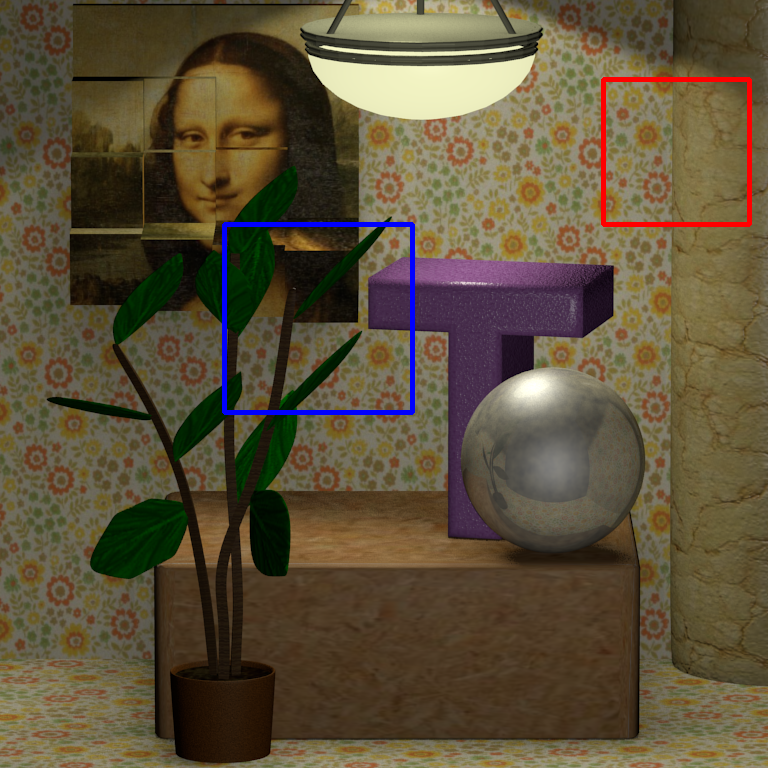
\includegraphics[width=0.22\textwidth, height=0.22\textwidth]{img/depth/full/monasRoom/rgb_annotated.png}
    } &
    
\includegraphics[width=0.110\textwidth, height=0.110\textwidth,cfbox=blue 1pt 0pt]{img/depth/crop/monasRoom/GT_1.png} &
    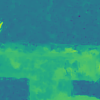
\includegraphics[width=0.110\textwidth, height=0.110\textwidth,cfbox=blue 1pt 0pt]{img/depth/crop/monasRoom/IINet_1.png} &
    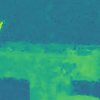
\includegraphics[width=0.110\textwidth, height=0.110\textwidth,cfbox=blue 1pt 0pt]{img/depth/crop/monasRoom/DistgSSR_1.png} &
    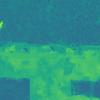
\includegraphics[width=0.110\textwidth, height=0.110\textwidth,cfbox=blue 1pt 0pt]{img/depth/crop/monasRoom/LFT_1.png} &
    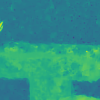
\includegraphics[width=0.110\textwidth, height=0.110\textwidth,cfbox=blue 1pt 0pt]{img/depth/crop/monasRoom/EPIT_1.png} &
    
\includegraphics[width=0.110\textwidth, height=0.110\textwidth,cfbox=blue 1pt 0pt]{img/depth/crop/monasRoom/SATNet_1.png} \\
    &
    
\includegraphics[width=0.110\textwidth, height=0.110\textwidth,cfbox=red 1pt 0pt]{img/depth/crop/monasRoom/GT_2.png} &
    
\includegraphics[width=0.110\textwidth, height=0.110\textwidth,cfbox=red 1pt 0pt]{img/depth/crop/monasRoom/IINet_2.png} &
    
\includegraphics[width=0.110\textwidth, height=0.110\textwidth,cfbox=red 1pt 0pt]{img/depth/crop/monasRoom/DistgSSR_2.png} &
    
\includegraphics[width=0.110\textwidth, height=0.110\textwidth,cfbox=red 1pt 0pt]{img/depth/crop/monasRoom/LFT_2.png} &
    \includegraphics[width=0.110\textwidth, height=0.110\textwidth,cfbox=red 1pt 0pt]{img/depth/crop/monasRoom/EPIT_2.png} &
    \includegraphics[width=0.110\textwidth, height=0.110\textwidth,cfbox=red 1pt 0pt]{img/depth/crop/monasRoom/SATNet_2.png} \\
    
    \textit{monasRoom} &
    Ground-truth &
    IINet \cite{liuLFIINet_TMM2021} &
    DistgSSR \cite{wangDistgSSR_TIP2022} &
    LFT \cite{liangLFT_SPL2022} &
    EPIT \cite{liangEPIT_arXiv2023} &
    M2MT-Net \\

    MSE$\times100$ &
    &
    0.584 &
    0.571 &
    0.590 &
    \underline{0.567} &
    \textbf{0.560} \\

    \end{tabular}
    }
    \caption{Visualization of depth estimation on the $4\times$ LFSR results of our M2MT-Net and the current state-of-the-art methods. Zoom-in depth maps are depicted on the areas in the blue and red boxes. MSE$\times 100$ is evaluated on the entire depth map. The best and second-best MSE are in bold and underlined.}
    \label{fig:Depth}
\end{figure*}
    

\subsection{Angular Consistency}
While the reconstruction of visual detail is important for LFSR, the preservation of parallax structure within LF images is equally crucial. This aspect of parallax structure cannot be adequately discerned solely by examining the reconstructed SAIs. Thus, to comprehensively assess the angular consistency, we conduct an evaluation through depth estimation. OACC-Net \cite{wangOACCNet_CVPR2022} is applied to generate depth maps on the super-resolved output of the methods under comparison. The depth estimated from HR images serves as the ground truth for this evaluation. Figure \ref{fig:Depth} visually represents the depth maps for two real-world and synthetic examples, accompanied by the $MSE\times100$ as a quantitative evaluation metric.

M2MT-Net's superiority, as highlighted in \textit{Perforated\_Metal\_3} of Figure \ref{fig:Qual}, is corroborated in the generated depth map. This method successfully reconstructs perforated holes with crisply integrated edges spanning from near to distant from the camera as evidenced in the blue and red boxes. In stark contrast, competing methods struggle, yielding blurred and entangled edges in this complex scene. When examining scenes featuring salient objects, M2MT-Net continues to excel. In the \textit{Sphynx} sample, the contours of the sphynx's nose, mouth and neck are distinctly delineated in M2MT-Net's depth map. Other methods, however, generate noticeable blurs or artifacts in these areas. The \textit{bicycle} sample further illustrates M2MT-Net's proficiency, where distinct separations between the bicycle's handlebar and the background are evident, as well as more continuous structures in the plant's trunks. Other methods falter, blending the handlebar's contour with the background or breaking the trunk's structure into fragments. Finally, in the \textit{monasRoom} example, M2MT-Net's depth map reveals a smoother surface on the T-shaped object and sharper contours on the leaf with fewer inaccuracies, demonstrating a closer approximation to the ground-truth when compared to the other methods, which produce noticeable bumpy artifacts.

These results collectively underscore M2MT-Net's leading capability not only in reconstructing visual details but also in preserving the parallax structure in super-resolved LF images, marking it as a significant advancement in LFSR.

\begin{table}[ht]
    \centering
    \caption{Comparison of computational efficiency against the state-of-the-art methods at the $4 \times$ scale. Runtime is the average elapsed time per sample over all 23 samples. \#Params is the number of trainable parameters.}
    \label{tab:efficiency}
    
    \begin{tabular}{|c|c|c|c|}
    \hline

    Method                                  & Type                  & Runtime/s   & \#Params   \\ \hline
    LF-IINet \cite{liuLFIINet_TMM2021}      & Convolution-based     & 1.34        & 4,885,824 \\
    DistgSSR \cite{wangDistgSSR_TIP2022}    & Convolution-based     & 1.70        & 3,581,568 \\
    LFT \cite{liangLFT_SPL2022}             & Transformer-based     & 5.84        & 1,163,392 \\
    EPIT \cite{liangEPIT_arXiv2023}         & Transformer-based     & 3.16        & 1,470,080 \\
    M2MT (Ours)                             & Transformer-based     & 2.03        & 3,986,400 \\
    \hline
    
    \end{tabular}
\end{table}
\begin{figure}[ht]
    \centering
    \tabcolsep=0.01cm
    \renewcommand{\arraystretch}{0.8}
    \begin{tabular}{c}
        \includegraphics[width=0.35\textwidth]{img/tradeoff/runtime.pdf} \\
        (a) PSNR vs Runtime \\
        \includegraphics[width=0.35\textwidth]{img/tradeoff/parameter.pdf} \\
        (b) PSNR vs Parameter Number
    \end{tabular}
    \caption{Tradeoff between performance and efficiency at the $4\times$ scale. The convolution-based methods are in red while the Transformer-based methods are in green. Candidates positioned closer to the top-right corner of the plots are better. }
    \label{fig:tradeoff}
\end{figure}


\subsection{Computational Efficiency}
We evaluate the computational efficiency of M2MT-Net against the best competitors LF-IINet, DistgSSR, LFT, and EPIT. Two metrics are involved: the running speed and the number of trainable parameters. The running speed measures the elapsed time per sample when running all 23 samples. The result is shown in Table \ref{tab:efficiency}, and the tradeoff between PSNR and runtime/parameter numbers is visualized as plots in Figure \ref{fig:tradeoff}. The convolution-based methods are in red while the Transformer-based methods are in green. In general, candidates positioned closer to the top-right corner of the plots indicate a more favorable tradeoff between performance and efficiency.

In terms of runtime, LF-IINet and DistgSSR are the fastest method as its convolution operations are local, making it quicker than global Transformer operations. Yet, within Transformer-based techniques, M2MT-Net emerges as the swiftest, taking approximately 20\% more time than DistgSSR but being 35\% and 65\% faster than EPIT and LFT respectively. This advantage is attributed to M2MT reducing the channel dimension from $UVC$ to $C_{Cor}$ via its linear layer in correlation encoding, significantly trimming the computational demand of the following self-attention component. On the flip side, this channel conversion makes M2MT bulkier in model size, as the linear layers require more parameters in both correlation encoding and decoding. Still, LF-SANet has 19\% fewer parameters than LF-IINet and 11\% more parameters than DistgSSR, keeping its size fairly manageable.

\subsection{Ablation Study}
In this section, we undertake a few ablation studies to understand the characteristic of M2MT-Net and its individual components. Note that the studies are carried out at the most challenging $4 \times$ scale using the \textit{EPFL} dataset as it has the most samples.

\subsubsection{Spatial and Angular Components}
To evaluate our proposed M2MT's role in the spatial subspace, we substitute it with a vanilla Transformer or a convolution and trained the network. The modified networks have similar sizes with the original M2MT-Net to ensure a fair comparison. As indicated in Table \ref{tab:ablation_altering}, substituting the M2MT with a vanilla Transformer deteriorates the performance by 0.51 dB to 29.29 dB. Opting for a convolution results in a further decline, with a drop of 0.78 dB to 29.02 dB. These outcomes affirm M2MT's efficacy as a feature extractor in the spatial subspace than other alternatives when paired with its angular subspace counterpart.

We also train a model replacing the angular Transformer with a convolution. Surprisingly, this variant achieves 29.42 dB PSNR, slightly outperforming Transformer-based competitors like LFT and EPIT. This underscores the robust adaptability of the M2MT, even when paired with less potent components.

\subsubsection{Number of Correlation Blocks}
We explore the performance of M2MT-Net with varying the number of correlation blocks $n_2$. Table \ref{tab:ablation_number_blocks} shows that M2MT-Net peaks in performance at $n_2 = 8$. Reducing the number leads to a gradual performance decline, and increasing it doesn't guarantee performance improvement due to the potential risk of overfitting.

\begin{table}[t!]
    \centering
    %\scriptsize
    \caption{Ablation study on altering components in correlation blocks. The best PSNR/SSIM are in bold.}
    \label{tab:ablation_altering}
    \resizebox{.45\textwidth}{!}{
    \begin{tabular}{|c|c|c|}
    \hline

    Spatial Component   &   Angular Component   & PSNR/SSIM \\ \hline
    M2MT                &   Vanilla Transformer & \textbf{29.80}/\textbf{0.9277} \\
    Vanilla Transformer &   Vanilla Transformer & 29.29/0.9213 \\
    Convolution         &   Vanilla Transformer & 29.02/0.9199 \\
    M2MT                &   Convolution         & 29.42/0.9208 \\
    % Convolution         &   Convolution         & 28.77/0.9135 \\
    \hline
    \end{tabular}
    }
\end{table}
\begin{table}[t!]
    \centering
    \caption{Ablation study on varing the number of correlation blocks. The best PSNR/SSIM are in bold.}
    \label{tab:ablation_number_blocks}
    \resizebox{.45\textwidth}{!}{
    \begin{tabular}{|c|c|c|c|c|c|}
    \hline

    % Number    & PSNR/SSIM \\ \hline
    % 6         & 29.49/0.9233 \\
    % 7         & 29.58/0.9239 \\
    % 8         & \textbf{29.67}/\textbf{0.9247} \\
    % 9         & 29.54/0.9223 \\
    % 10        & 29.60/\textbf{0.9247} \\

    Number    & 6       & 7         & 8                 & 9         & 10        \\ \hline
    PSNR      & 29.60   & 29.69     & \textbf{29.80}    & 29.65     & 29.66     \\
    SSIM      & 0.9257  & 0.9270    & \textbf{0.9277}   & 0.9270    & 0.9271    \\
    \hline
    
    \end{tabular}
    }
\end{table}